\clearpage
\VerdierPhysicalPageAnchor{0133}%
\begingroup
\small
\setlength{\emergencystretch}{1.5em}%
\setlength{\abovedisplayskip}{1pt plus 1pt minus 1pt}%
\setlength{\belowdisplayskip}{1pt plus 1pt minus 1pt}%
\newcommand{\VerdierHatchTriangle}[3]{%
  \begin{scope}
    \clip (#1) -- (#2) -- (#3) -- cycle;
    \draw[step=.20cm,black!78,line width=.16pt] (-2,-2) grid (7,2);
  \end{scope}}

\VerdierSemanticAnchor{ch2-2-1-13}
\noindent\textbf{2.1.13.}\quad
\VerdierSemanticAnchor{ch2-2-1-13-saturation-direction}%
\emph{如果范畴 $\mathcal D'$ 是饱和的，则集合 $S(\mathcal D')$ 是饱和的。}
\VerdierSemanticAnchor{ch2-2-1-13-composable-setup}%
设 $f,g,h$ 为三个可复合态射，使 $fg$ 与 $gh$ 都属于 $S(\mathcal D')$。

\VerdierSemanticAnchor{ch2-2-1-13-triv-construction}
利用公理 TRIV，可以构造图式：

\VerdierSemanticAnchor{ch2-2-1-13-triv-diagram}
\begin{center}
  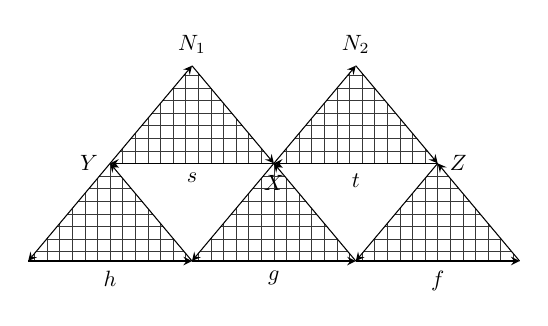
\begin{tikzpicture}[>=stealth,line width=.38pt,scale=.80,transform shape]
    \coordinate (Y)  at (0,0);
    \coordinate (X)  at (2.6,0);
    \coordinate (Z)  at (5.2,0);
    \coordinate (N1) at (1.3,1.55);
    \coordinate (N2) at (3.9,1.55);
    \coordinate (A)  at (-1.3,-1.55);
    \coordinate (Q1) at (1.3,-1.55);
    \coordinate (Q2) at (3.9,-1.55);
    \coordinate (B)  at (6.5,-1.55);

    \VerdierHatchTriangle{Y}{N1}{X}
    \VerdierHatchTriangle{X}{N2}{Z}
    \VerdierHatchTriangle{Y}{A}{Q1}
    \VerdierHatchTriangle{X}{Q1}{Q2}
    \VerdierHatchTriangle{Z}{Q2}{B}

    \draw[->] (Y) -- (N1);
    \draw[->] (N1) -- (X);
    \draw[->] (X) -- node[below=1pt] {$s$} (Y);
    \draw[->] (X) -- (N2);
    \draw[->] (N2) -- (Z);
    \draw[->] (Z) -- node[below=1pt] {$t$} (X);

    \draw[->] (Y) -- (A);
    \draw[->] (A) -- node[below=1pt] {$h$} (Q1);
    \draw[->] (Q1) -- (Y);
    \draw[->] (X) -- (Q1);
    \draw[->] (Q1) -- node[below=1pt] {$g$} (Q2);
    \draw[->] (Q2) -- (X);
    \draw[->] (Z) -- (Q2);
    \draw[->] (Q2) -- node[below=1pt] {$f$} (B);
    \draw[->] (B) -- (Z);

    \node[left=2pt]  at (Y)  {$Y$};
    \node[below=2pt] at (X)  {$X$};
    \node[right=2pt] at (Z)  {$Z$};
    \node[above=2pt] at (N1) {$N_1$};
    \node[above=2pt] at (N2) {$N_2$};
  \end{tikzpicture}
  \quad ,
\end{center}

\VerdierSemanticAnchor{ch2-2-1-13-diagram-interpretation}
\noindent 其中 $N_1$ 与 $N_2$ 是 $\mathcal D'$ 的对象，五个带阴影的三角是
特异三角，两个未带阴影的三角是交换的。

\VerdierSemanticAnchor{ch2-2-1-13-shifted-zero}
由此得到 $s[1]t=0$ (1.2.2)。
\VerdierSemanticAnchor{ch2-2-1-13-shifted-membership}%
此外，由 SM1) 与 SM5)，态射 $s[1]t$ 属于 $S(\mathcal D')$。

\VerdierSemanticAnchor{ch2-2-1-13-split-triangle}
因此存在形如 $(Z,Y[2],N,0,u,v)$ 的特异三角，其中 $N$ 是 $\mathcal D'$
的对象。
\VerdierSemanticAnchor{ch2-2-1-13-direct-summand}%
由 (1.2.6) 与 TRII 可知，$Y$ 是 $\mathcal D'$ 的某个对象的直和项。
\VerdierSemanticAnchor{ch2-2-1-13-y-in-dprime}%
因此，$Y$ 同构于 $\mathcal D'$ 的一个对象。

\VerdierSemanticAnchor{ch2-2-1-13-s-triangle}
再利用 (1.2.4)、$\mathcal D'$ 是 $\mathcal D$ 的三角子范畴这一事实，以及
特异三角：

\begin{center}
  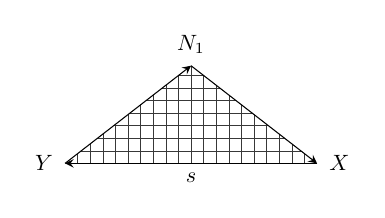
\begin{tikzpicture}[>=stealth,line width=.38pt,scale=.80,transform shape]
    \coordinate (Y)  at (-2,0);
    \coordinate (X)  at (2,0);
    \coordinate (N1) at (0,1.55);
    \VerdierHatchTriangle{Y}{N1}{X}
    \draw[->] (Y) -- (N1);
    \draw[->] (N1) -- (X);
    \draw[->] (X) -- node[below=1pt] {$s$} (Y);
    \node[left=2pt]  at (Y)  {$Y$};
    \node[right=2pt] at (X)  {$X$};
    \node[above=2pt] at (N1) {$N_1$};
  \end{tikzpicture}
\end{center}

\VerdierSemanticAnchor{ch2-2-1-13-g-membership}
\noindent 可知 $X$ 同构于 $\mathcal D'$ 的一个对象。因此，态射 $g$ 属于
$S(\mathcal D')$。

\VerdierSemanticAnchor{ch2-2-1-14}
\medskip
\noindent\textbf{2.1.14.}\quad
\VerdierSemanticAnchor{ch2-2-1-14-saturation-direction}%
\emph{如果集合 $S(\mathcal D')$ 是饱和的，则子范畴 $\mathcal D'$ 是饱和的。}

\VerdierSemanticAnchor{ch2-2-1-14-direct-summand-setup}
设 $X$ 为 $\mathcal D'$ 的某个对象的直和项。
\VerdierSemanticAnchor{ch2-2-1-14-first-triangle}%
由 (1.2.6) 与 TRII 可见，存在特异三角 $(X,Y,N,0,u,v)$，其中 $N$ 是
$\mathcal D'$ 的对象。
\VerdierSemanticAnchor{ch2-2-1-14-zero-morphism}%
因此，零态射 $X\to Y$ 属于 $S(\mathcal D')$。

\VerdierSemanticAnchor{ch2-2-1-14-sm4-application}
把性质 SM4) 应用于三个态射 $0\to X\to 0\to Y$。
\VerdierSemanticAnchor{ch2-2-1-14-x-zero-membership}%
由此可知态射 $X\to 0$ 属于 $S(\mathcal D')$。

\VerdierSemanticAnchor{ch2-2-1-14-second-triangle}
因此存在特异三角 $(X,0,N,0,0,i)$，其中 $N$ 是 $\mathcal D'$ 的对象。
\VerdierSemanticAnchor{ch2-2-1-14-shift-isomorphism}%
于是态射 $N\xrightarrow{i}X[1]$ 是同构。因此 $X$ 同构于 $N[-1]$，
而后者是 $\mathcal D'$ 的对象。

\VerdierSemanticAnchor{ch2-2-1-14-proposition-complete}
这就完成了命题 (2.1.8) 的证明。

\VerdierSemanticAnchor{ch2-2-1-14-p134-boundary}
\endgroup
